\documentclass[aspectratio=169,11pt]{beamer}
\usetheme{default}
\usefonttheme{serif}
\setbeamertemplate{navigation symbols}{}
\setbeamertemplate{footline}[frame number]
\setbeamertemplate{itemize items}[circle]
\setbeamersize{text margin left=10mm,text margin right=10mm}
\usepackage{fontspec}
\usepackage{unicode-math}
\setmainfont{texgyrepagella}[Path=fonts/, Extension=.otf,
  UprightFont=*-regular, ItalicFont=*-italic,
  BoldFont=*-bold, BoldItalicFont=*-bolditalic]
\setmathfont{texgyrepagella-math}[Path=fonts/, Extension=.otf]
% Pagella uses U+2216 for set difference.
\AtBeginDocument{\let\setminus\smallsetminus}
\usepackage{array,booktabs}
\usepackage{tikz}
\usetikzlibrary{arrows.meta,positioning,calc}
\definecolor{arb}{RGB}{27,94,52}
\definecolor{arbred}{RGB}{150,40,40}
\definecolor{arbdim}{RGB}{100,100,100}
\setbeamercolor{structure}{fg=arb}
\setbeamercolor{frametitle}{fg=arb}
\setbeamercolor{alerted text}{fg=arbred}
\setbeamerfont{frametitle}{size=\Large,series=\bfseries}
\setbeamerfont{title}{size=\huge,series=\bfseries}

\newcommand{\F}{\mathbb{F}}
\newcommand{\G}{\mathbb{G}}
\newcommand{\Ep}{\ensuremath{\mathcal{E}}}
\newcommand{\Pallas}{\ensuremath{\mathsf{Pallas}}}
\newcommand{\Vesta}{\ensuremath{\mathsf{Vesta}}}
\newcommand{\Fpp}{\ensuremath{\F_{p}}}
\newcommand{\nfsym}{\ensuremath{\mathsf{nf}}}
\newcommand{\cmsym}{\ensuremath{\mathsf{cm}}}
\newcommand{\cmx}{\ensuremath{\mathsf{cmx}}}
\newcommand{\cvsym}{\ensuremath{\mathsf{cv}}}
\newcommand{\rksym}{\ensuremath{\mathsf{rk}}}
\newcommand{\gd}{\ensuremath{\mathsf{g_d}}}
\newcommand{\pkd}{\ensuremath{\mathsf{pk_d}}}
\newcommand{\aksym}{\ensuremath{\mathsf{ak}}}
\newcommand{\nksym}{\ensuremath{\mathsf{nk}}}
\newcommand{\asksym}{\ensuremath{\mathsf{ask}}}
\newcommand{\ivk}{\ensuremath{\mathsf{ivk}}}
\newcommand{\fvk}{\ensuremath{\mathsf{fvk}}}
\newcommand{\ovk}{\ensuremath{\mathsf{ovk}}}
\newcommand{\dk}{\ensuremath{\mathsf{dk}}}
\newcommand{\rcm}{\ensuremath{\mathsf{rcm}}}
\newcommand{\rcv}{\ensuremath{\mathsf{rcv}}}
\newcommand{\rivk}{\ensuremath{\mathsf{r_{ivk}}}}
\newcommand{\rsk}{\ensuremath{\mathsf{rsk}}}
\newcommand{\esk}{\ensuremath{\mathsf{esk}}}
\newcommand{\epk}{\ensuremath{\mathsf{epk}}}
\newcommand{\Extract}{\ensuremath{\mathsf{Extract}}}
\newcommand{\NoteCommit}{\ensuremath{\mathsf{NoteCommit}}}
\newcommand{\GroupHash}{\ensuremath{\mathsf{GroupHash}}}
\newcommand{\CommitIvk}{\ensuremath{\mathsf{Commit}^{\mathsf{ivk}}}}
\newcommand{\ip}[2]{\langle #1,\, #2 \rangle}
\newcommand{\bvk}{\ensuremath{\mathsf{bvk}}}
\newcommand{\bsk}{\ensuremath{\mathsf{bsk}}}
\newcommand{\vbal}{\ensuremath{v_{\mathrm{balance}}}}
\newcommand{\Ecenc}{\ensuremath{C_{\mathrm{enc}}}}
\newcommand{\Ecout}{\ensuremath{C_{\mathrm{out}}}}
\newcommand{\Ecv}{\ensuremath{\cvsym}}
\newcommand{\Enf}{\ensuremath{\nfsym}}
\newcommand{\Eanc}{\ensuremath{\mathsf{anchor}}}
\newcommand{\Dint}[1]{\ensuremath{#1^{\mathsf{int}}}}
\newcommand{\Dprf}[1]{\ensuremath{\mathsf{PRFexpand}_{#1}}}
\newcommand{\Dff}{\ensuremath{\mathsf{FF1}}}
\newcommand{\GZH}{\ensuremath{Z_H}}
\newcommand{\Glo}[1]{\ensuremath{#1_{\mathrm{lo}}}}
\newcommand{\Ghi}[1]{\ensuremath{#1_{\mathrm{hi}}}}

\definecolor{tierfull}{RGB}{210,140,40}
\definecolor{tierin}{RGB}{60,130,180}
\definecolor{tierspend}{RGB}{200,60,60}
\definecolor{tierrecv}{RGB}{70,150,90}
\tikzset{
  keykn/.style={draw=#1, fill=#1, fill opacity=0.14, text opacity=1,
    line width=0.7pt, rounded corners=2pt, inner sep=3pt,
    minimum height=6mm, minimum width=9mm, align=center},
  keyix/.style={draw=gray, line width=0.7pt, rounded corners=2pt,
    inner sep=3pt, minimum height=6mm, align=center},
  keyed/.style={->, line width=0.6pt},
  keylb/.style={font=\scriptsize, inner sep=1.5pt, align=center}}
\tikzset{box/.style={draw=arb,rounded corners,inner sep=4pt,align=center,font=\small},
  flow/.style={-{Stealth[length=2mm]},thick,arb},
  labeltext/.style={font=\small,text=arbdim,align=center}}
\newcommand{\divider}[1]{\begin{frame}[plain]\vfill\centering
  {\usebeamercolor[fg]{structure}\Huge\bfseries #1}\vfill\end{frame}}
\newcommand{\grey}[1]{{\color{arbdim}#1}}
\newcommand{\types}[1]{\par\smallskip{\small\color{arbdim}#1}\par}
\newcommand{\PP}{\mathbb{P}}
\newcommand{\pP}{p_{\mathsf{Pallas}}}
\newcommand{\pV}{p_{\mathsf{Vesta}}}
\newcommand{\FP}{\F_{\pP}}
\newcommand{\FV}{\F_{\pV}}
\newcommand{\EP}{\Ep(\FP)}
\newcommand{\Ext}{\Extract_{\PP}}
\newcommand{\akP}{\aksym^{\PP}}
\newcommand{\rk}{\rksym}
\newcommand{\sksym}{\mathsf{sk}}
\newcommand{\Hs}{\mathsf{H}^{\circledast}}
\newcommand{\PRFx}[1]{\mathsf{PRFexpand}_{#1}}
\newcommand{\LE}[1]{\mathrm{LE}_{#1}}
\newcommand{\Ilep}[1]{\mathsf{I2LEOSP}_{#1}}
\newcommand{\SinHash}{\mathsf{SinsemillaHash}}
\newcommand{\SinPt}{\mathsf{SinsemillaHashToPoint}}
\newcommand{\SinCom}{\mathsf{SinsemillaCommit}}
\newcommand{\ShortCom}{\mathsf{ShortCommit}}
\newcommand{\MCRH}{\mathsf{MerkleCRH}}
\newcommand{\DivH}{\mathsf{DiversifyHash}}
\newcommand{\DNf}{\mathsf{DeriveNullifier}}
\newcommand{\VC}{\mathsf{ValueCommit}}
\newcommand{\VO}{V^{\mathsf{Orchard}}}
\newcommand{\RO}{R^{\mathsf{Orchard}}}
\newcommand{\KO}{K^{\mathsf{Orchard}}}
\newcommand{\GS}{G^{\mathsf{SpendAuth}}}
\newcommand{\vnet}{v^{\mathsf{net}}}
\newcommand{\cvnet}{\cvsym^{\mathsf{net}}}
\newcommand{\vb}{v^{\mathsf{balance}}}
\newcommand{\old}{^{\mathsf{old}}}
\newcommand{\new}{^{\mathsf{new}}}
\newcommand{\rseed}{\mathsf{rseed}}
\newcommand{\ZH}{Z_H}
\newcommand{\Rel}{\mathcal{R}}
\newcommand{\bfa}{\mathbf{a}}
\newcommand{\bfb}{\mathbf{b}}
\newcommand{\bfG}{\mathbf{G}}
\newcommand{\lo}{\mathrm{lo}}
\newcommand{\hi}{\mathrm{hi}}
\newcommand{\Vs}{\ensuremath{\mathcal{V}}}
\newcommand{\rtag}[1]{\hfill{\small\color{arbdim}#1}}
\newcommand{\stmt}[2]{\par\smallskip\noindent\textbf{#1}\enspace\textit{#2}\par}
\newcommand{\proofidea}[1]{\par\smallskip\noindent{\small\textit{Proof.}\enspace #1}\par}
% ---- The commitment tree (depth 3 toy; the real tree has depth 32).
\newcommand{\CTreeMode}{none}
\newcommand{\CTreeAnchor}{anchor}
\newcommand{\CTreeLeaf}{leaf}
\newcommand{\CTreePath}{path}
\newcommand{\TreeFig}[1][none]{%
  \renewcommand{\CTreeMode}{#1}%
  \tikzset{croot/.style={},cleaf/.style={},croute/.style={},
    csib/.style={},cedge/.style={}}%
  \ifx\CTreeMode\CTreeAnchor\tikzset{croot/.style={chl}}\fi
  \ifx\CTreeMode\CTreeLeaf\tikzset{cleaf/.style={chl}}\fi
  \ifx\CTreeMode\CTreePath\tikzset{cleaf/.style={chl},croute/.style={chl},
    csib/.style={fill=arb!25},cedge/.style={draw=arbred,very thick}}\fi
  \begin{tikzpicture}[x=7.2mm,y=7.5mm,every node/.style={font=\scriptsize},
    lf/.style={draw,minimum width=6mm,minimum height=4mm,inner sep=1pt},
    nd/.style={draw,circle,inner sep=1.6pt},
    ed/.style={black!55},
    chl/.style={draw=arbred,very thick,fill=arbred!15}]
  \node[lf] (L0) at (0,0) {\cmx};
  \node[lf] (L1) at (1,0) {\cmx};
  \node[lf,cleaf] (L2) at (2,0) {\cmx};
  \node[lf,csib] (L3) at (3,0) {\cmx};
  \node[lf] (L4) at (4,0) {\cmx};
  \node[lf] (L5) at (5,0) {\cmx};
  \node[lf] (L6) at (6,0) {\cmx};
  \node[lf,dashed] (L7) at (7,0) {$\varnothing$};
  \node[nd,csib] (A) at (0.5,1) {};
  \node[nd,croute] (B) at (2.5,1) {};
  \node[nd] (C) at (4.5,1) {};
  \node[nd] (D) at (6.5,1) {};
  \node[nd,croute] (E) at (1.5,2) {};
  \node[nd,csib] (F) at (5.5,2) {};
  \node[draw,rounded corners,fill=arb!15,croot] (R) at (3.5,3) {anchor};
  \draw[ed] (A)--(L0); \draw[ed] (A)--(L1); \draw[ed] (B)--(L3);
  \draw[ed] (C)--(L4); \draw[ed] (C)--(L5); \draw[ed] (D)--(L6);
  \draw[ed] (D)--(L7); \draw[ed] (E)--(A); \draw[ed] (F)--(C);
  \draw[ed] (F)--(D); \draw[ed] (R)--(F);
  \draw[ed,cedge] (L2)--(B); \draw[ed,cedge] (B)--(E);
  \draw[ed,cedge] (E)--(R);
  \ifx\CTreeMode\CTreeLeaf
    \node[text=arbred,below=1pt of L2] {$p$};\fi
  \ifx\CTreeMode\CTreePath
    \node[text=arbred,below=1pt of L2] {$p$};\fi
  \end{tikzpicture}}

% ---- One Action inside its bundle.
\newcommand{\ActionBox}[1][none]{%
  \tikzset{hlnone/.style={}, hlanchor/.style={}, hlnf/.style={},
    hlcv/.style={}, hlrk/.style={}, hlcmx/.style={}, hlproof/.style={},
    hl#1/.style={draw=arbred, very thick, fill=arbred!15}}%
  \begin{tikzpicture}[font=\scriptsize, x=1cm, y=1cm,
    ebox/.style={draw=black!60, fill=white, rounded corners=2pt,
      inner sep=2.5pt, align=center},
    elab/.style={inner sep=2pt, text=black!60}]
  \draw[draw=black!50, dashed, rounded corners=3pt]
    (-2.45,-2.45) rectangle (4.75,2.5);
  \node[elab, anchor=north west, text=black!70, font=\scriptsize\bfseries]
    at (-2.45,2.5) {bundle};
  \draw[draw=arb!40, rounded corners=3pt] (-2.0,-2.1) rectangle (2.4,2.1);
  \node[elab, anchor=south east, text=arb!60] at (2.4,2.1) {$\times\,n$};
  \node[draw=arb, thick, fill=white, rounded corners=3pt,
    minimum width=4.4cm, minimum height=3.9cm] (act) at (0,0) {};
  \node[anchor=north west, font=\scriptsize\bfseries, text=arb,
    inner sep=2pt] at (act.north west) {Action};
  \node[draw=arb!60, fill=arb!8, rounded corners=2pt, inner sep=3pt,
    align=center, anchor=north, text width=3.8cm] (wit) at (0,1.62)
    {\textbf{witness} --- never published\\
     old note, new note\\
     Merkle path $+$ position\\
     $\aksym, \nksym, \rivk, \ivk$; $\alpha$, $\rcv$};
  \node[elab, anchor=west] at (-2.15,-0.12) {public, per Action};
  \node[ebox, hlcv, anchor=west] (cv) at (-2.05,-0.58) {$\Ecv$};
  \node[ebox, hlnf, right=1.2mm of cv] (nf) {$\Enf$};
  \node[ebox, hlrk, right=1.2mm of nf] (rk) {$\rksym$};
  \node[ebox, hlcmx, right=1.2mm of rk] (cmx) {$\cmx$};
  \node[ebox, draw=black!40, dashed] (ct) at (0,-1.15)
    {$\epk,\ \Ecenc,\ \Ecout$};
  \node[elab, align=center, font=\tiny, text=black!60] at (0,-1.66)
    {delivery ciphertexts --- opened only with $\ivk$ / $\ovk$};
  \node[ebox, hlanchor, anchor=west] (anc) at (2.45,1.65) {$\Eanc$};
  \node[ebox, anchor=west] (flg) at (2.45,1.0) {flags};
  \node[ebox, anchor=west] (vb)  at (2.45,0.35) {$\vbal$};
  \node[ebox, hlproof, anchor=west] (prf) at (2.45,-0.3) {proof};
  \node[ebox, anchor=west] (sas) at (2.45,-0.95) {SpendAuthSigs};
  \node[ebox, anchor=west] (bsg) at (2.45,-1.6) {binding sig};
  \end{tikzpicture}}


% ---- The key ladder, in the notation of the Ironwood Guide.
\newcommand{\LadderFig}{%
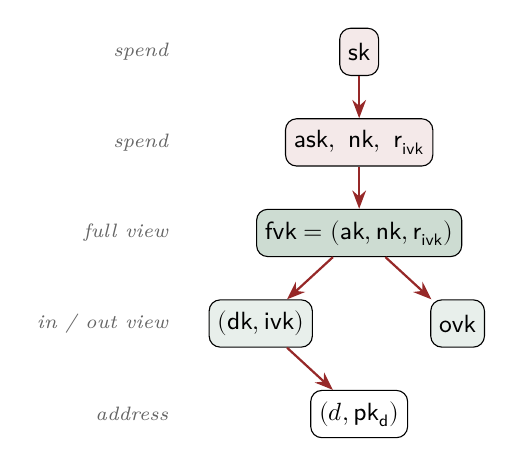
\begin{tikzpicture}[font=\small, x=1cm, y=1cm,
  k/.style={draw, rounded corners, inner sep=3pt, minimum height=6mm,
            anchor=center, fill=arb!10},
  kspend/.style={k, fill=arbred!10},
  kfull/.style={k, fill=arb!22},
  kpub/.style={k, fill=white},
  tier/.style={font=\scriptsize\itshape, text=arbdim, anchor=east},
  op/.style={font=\footnotesize, anchor=west, align=left},
  ow/.style={-{Stealth}, thick, arbred}]
\node[kspend] (sk)  at (0,0)     {$\sksym$};
\node[kspend] (mid) at (0,-1.15) {$\asksym,\ \nksym,\ \rivk$};
\node[kfull]  (fvk) at (0,-2.3)  {$\fvk = (\aksym, \nksym, \rivk)$};
\node[k]      (ivk) at (-1.25,-3.45) {$(\dk, \ivk)$};
\node[k]      (ovk) at (1.25,-3.45)  {$\ovk$};
\node[kpub]   (adr) at (0,-4.6)  {$(d, \pkd)$};
\draw[ow] (sk) -- (mid); \draw[ow] (mid) -- (fvk);
\draw[ow] (fvk) -- (ivk); \draw[ow] (fvk) -- (ovk);
\draw[ow] (ivk) -- (adr);
\node[tier] at (-2.3,0)     {spend};
\node[tier] at (-2.3,-1.15) {spend};
\node[tier] at (-2.3,-2.3)  {full view};
\node[tier] at (-2.3,-3.45) {in / out view};
\node[tier] at (-2.3,-4.6)  {address};
\end{tikzpicture}}

% ---- The deficit walk: two seeded runs from z = 2.
\newcommand{\Kwalk}{%
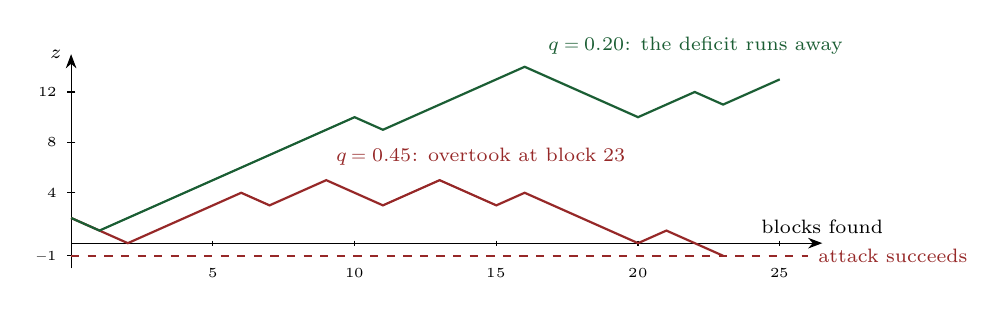
\begin{tikzpicture}[x=0.36cm, y=0.16cm]
\draw[-{Stealth[length=1.8mm]}] (0,-2) -- (0,15)
  node[left, font=\scriptsize] {$z$};
\draw[-{Stealth[length=1.8mm]}] (0,0) -- (26.5,0)
  node[above, font=\scriptsize] {blocks found};
\foreach \y in {-1, 4, 8, 12}
  \draw (0.15,\y) -- (-0.15,\y) node[left, font=\tiny] {$\y$};
\draw[dashed, thick, arbred] (0,-1) -- (26,-1)
  node[right, font=\scriptsize, text=arbred] {attack succeeds};
\foreach \x in {5, 10, 15, 20, 25} {
  \draw (\x,0.2) -- (\x,-0.2);
  \node[below, font=\tiny] at (\x,-1.2) {$\x$};
}
\draw[thick, arbred] plot coordinates {(0,2) (1,1) (2,0) (3,1) (4,2)
  (5,3) (6,4) (7,3) (8,4) (9,5) (10,4) (11,3) (12,4) (13,5) (14,4)
  (15,3) (16,4) (17,3) (18,2) (19,1) (20,0) (21,1) (22,0) (23,-1)};
\node[font=\scriptsize, text=arbred, anchor=south west] at (9,5.4)
  {$q = 0.45$: overtook at block $23$};
\draw[thick, arb] plot coordinates {(0,2) (1,1) (2,2) (3,3) (4,4) (5,5)
  (6,6) (7,7) (8,8) (9,9) (10,10) (11,9) (12,10) (13,11) (14,12) (15,13)
  (16,14) (17,13) (18,12) (19,11) (20,10) (21,11) (22,12) (23,11)
  (24,12) (25,13)};
\node[font=\scriptsize, text=arb, anchor=south west] at (16.5,14.2)
  {$q = 0.20$: the deficit runs away};
\end{tikzpicture}}


\title{Zcash, end to end}
\subtitle{from a wallet seed to a verified shielded payment}
\author{m@rek.onl}
\date{}

\begin{document}

\begin{frame}[plain]
\titlepage
\end{frame}

% ====================================================================
\divider{One order}

\begin{frame}{Why nodes must agree on an order}
Two transactions spend the same coin. Each is valid alone; together, one
must lose.
\vfill
\begin{center}
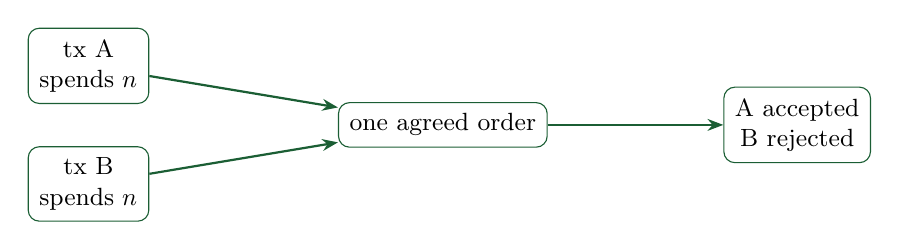
\begin{tikzpicture}[x=1cm,y=1cm]
\node[box] (a) at (0,0) {tx A\\spends $n$};
\node[box] (b) at (0,-1.5) {tx B\\spends $n$};
\node[box] (o) at (4.5,-0.75) {one agreed order};
\node[box] (r) at (9,-0.75) {A accepted\\B rejected};
\draw[flow] (a) -- (o); \draw[flow] (b) -- (o); \draw[flow] (o) -- (r);
\end{tikzpicture}
\end{center}
\vfill
Consensus supplies a \textbf{canonical order}: the chain with the most
work. Every later rule, the note tree, the nullifier set, the pool
balances, is a function of that order.
\end{frame}

\begin{frame}{The race}
An attacker mines a secret branch; $z$ is the honest chain's lead in blocks.
\[
z_{i+1} = \begin{cases} z_i + 1 & \text{honest block, probability } p \\
z_i - 1 & \text{attacker block, probability } q = 1 - p \end{cases}
\]
The attack succeeds when $z$ reaches $-1$.
\vfill
\begin{center}
\Kwalk
\end{center}
\end{frame}

\begin{frame}{Deriving the catch-up probability}
Let $h_N(z)$ be the probability that the walk from $z$ reaches $-1$ before
a ceiling $N$. Condition on the next block:
\[
h_N(z) = p\,h_N(z+1) + q\,h_N(z-1), \qquad h_N(-1) = 1, \quad h_N(N) = 0 .
\]
The trial solution $h_N(z) = t^z$ works exactly at the roots of
\[
p\,t^2 - t + q = p\,(t - 1)\,(t - q/p) ,
\]
so for $q \ne p$, $h_N(z) = A + B\,(q/p)^z$, and the two boundaries give
\[
h_N(z) = \frac{(q/p)^z - (q/p)^N}{(q/p)^{-1} - (q/p)^N}
\;\xrightarrow{\;N \to \infty\;}\; a_z = (q/p)^{z+1} \qquad (q < p).
\]
For $q \ge p$ the limit is $1$: an attacker with half the hashrate or more
always catches up.
\end{frame}

\begin{frame}{The catch-up probability}
\[
a_z = \Pr[\text{the walk ever reaches } {-1} \text{ from } z]
  = \begin{cases} (q/p)^{z+1} & q < p \\ 1 & q \ge p \end{cases}
\]
\begin{columns}[c]
\begin{column}{0.56\textwidth}
\centering
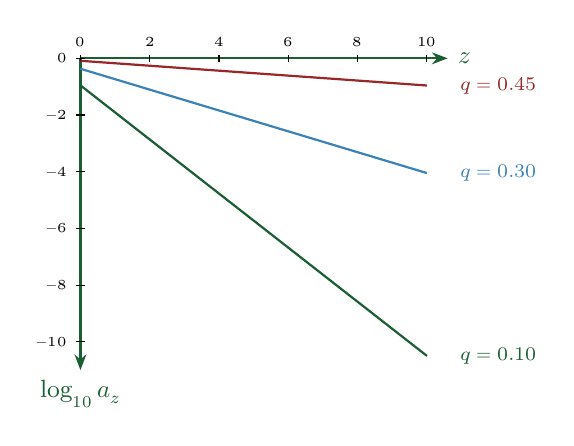
\begin{tikzpicture}[x=0.44cm, y=0.36cm]
\draw[flow] (0,0) -- (10.6,0) node[right, font=\small] {$z$};
\draw[flow] (0,0) -- (0,-11) node[below, font=\small] {$\log_{10} a_z$};
\foreach \y in {0,-2,-4,-6,-8,-10}
  \draw (0.12,\y) -- (-0.12,\y) node[left, font=\tiny] {$\y$};
\foreach \x in {0,2,4,6,8,10}
  \draw (\x,0.12) -- (\x,-0.12) node[above=2pt, font=\tiny] {$\x$};
\draw[thick, arb] plot coordinates {(0,-0.954) (1,-1.908) (2,-2.863)
  (3,-3.817) (4,-4.771) (5,-5.725) (6,-6.680) (7,-7.634) (8,-8.588)
  (9,-9.542) (10,-10.497)};
\draw[thick, tierin] plot coordinates {(0,-0.368) (1,-0.736) (2,-1.104)
  (3,-1.472) (4,-1.840) (5,-2.208) (6,-2.576) (7,-2.944) (8,-3.312)
  (9,-3.680) (10,-4.048)};
\draw[thick, arbred] plot coordinates {(0,-0.087) (1,-0.174) (2,-0.261)
  (3,-0.349) (4,-0.436) (5,-0.523) (6,-0.610) (7,-0.697) (8,-0.784)
  (9,-0.872) (10,-0.959)};
\node[font=\scriptsize, text=arb, anchor=west] at (10.7,-10.5) {$q = 0.10$};
\node[font=\scriptsize, text=tierin, anchor=west] at (10.7,-4.05) {$q = 0.30$};
\node[font=\scriptsize, text=arbred, anchor=west] at (10.7,-0.96) {$q = 0.45$};
\end{tikzpicture}
\end{column}
\begin{column}{0.42\textwidth}
\small
\begin{tabular}{@{}lll@{}}
\toprule
$q$ & $a_0$ & $a_5$ \\
\midrule
$0.10$ & $0.111$ & $1.9 \times 10^{-6}$ \\
$0.30$ & $0.429$ & $6.2 \times 10^{-3}$ \\
$0.45$ & $0.818$ & $0.30$ \\
\bottomrule
\end{tabular}
\par\bigskip
Each block of lead multiplies $a_z$ by $q/p$: the order of old blocks
becomes final exponentially fast.
\end{column}
\end{columns}
\end{frame}

\begin{frame}{What the order gives the shielded protocol}
\begin{center}
\begin{tabular}{@{}ll@{}}
\toprule
object & a function of the ordered chain \\
\midrule
note commitment tree & every $\cmx$, appended in order \\
anchor & the tree's root after a block \\
nullifier set & every $\nfsym$ published so far \\
pool balance & minus the sum of every $\vbal$ \\
\bottomrule
\end{tabular}
\end{center}
\vfill
From here on: one canonical chain. The rest of the talk follows one
payment through it.
\end{frame}

% ====================================================================
\divider{Keys}

\begin{frame}{From the seed to an account key}
\[
I := \mathrm{BLAKE2b\text{-}512}(\texttt{ZcashIP32Orchard},\, S),\qquad
(\sksym_m, c_m) := (I[0..32),\ I[32..64))
\]
\[
(\sksym_i, c_i) := \PRFx{c_{\mathrm{par}}}\bigl([\mathtt{0x81}] \,\|\,
  \sksym_{\mathrm{par}} \,\|\, \Ilep{32}(i)\bigr) \quad\text{split in halves},
  \quad i \ge 2^{31}
\]
\vfill
Path $m / 32' / 133' / a'$ (purpose, coin type, account):
\begin{center}\small
\begin{tabular}{@{}ll@{}}
\toprule
node & spending key $\sksym$ \\
\midrule
$m$ & \texttt{7eee3c10\dots8e8b2cd4b8} \\
$m/32'$ & \texttt{93af0a87\dots2dc9eb0f87} \\
$m/32'/133'$ & \texttt{149fcee5\dots1a0bcb0e8c4c} \\
$m/32'/133'/0'$ & \texttt{b67d8d87\dots8313cb223b4} \\
\bottomrule
\end{tabular}
\end{center}
\types{$S$ the seed bytes $\mathtt{00}, \dots, \mathtt{1f}$; every step is
one-way and hardened.}
\end{frame}

\begin{frame}{Spending secrets}
\begin{align*}
\asksym &:= \mathrm{ToScalar}\bigl(\PRFx{\sksym}([\mathtt{06}])\bigr) \in \FV \\
\nksym &:= \mathrm{ToBase}\bigl(\PRFx{\sksym}([\mathtt{07}])\bigr) \in \FP \\
\rivk &:= \mathrm{ToScalar}\bigl(\PRFx{\sksym}([\mathtt{08}])\bigr) \in \FV
\end{align*}
\[
\akP := [\asksym]\,\GS \in \EP \quad\text{(even } y\text{)},\qquad
\aksym := \Ext(\akP)
\]
\vfill
$\asksym$ signs spends; $\nksym$ keys nullifiers; $\rivk$ blinds the
viewing key.
\types{$\PRFx{k}$ is BLAKE2b-512 personalised \texttt{Zcash\_ExpandSeed}; the
lead byte names the output.}
\end{frame}

\begin{frame}{Viewing keys}
\[
\ivk := \CommitIvk_{\rivk}(\aksym, \nksym)
  = \Ext\bigl(\SinPt(\aksym \,\|\, \nksym) + [\rivk]\,H\bigr)
\]
\[
\dk \,\|\, \ovk := \PRFx{\rivk}\bigl([\mathtt{82}] \,\|\, \aksym \,\|\, \nksym\bigr)
\]
\vfill
\begin{center}
\begin{tabular}{@{}ll@{}}
\toprule
key & lets its holder \\
\midrule
$\asksym$ & spend \\
$(\aksym, \nksym, \rivk)$ & see spends (nullifiers) \\
$(\dk, \ivk)$ & see incoming notes, make addresses \\
$\ovk$ & recover what it sent \\
\bottomrule
\end{tabular}
\end{center}
\end{frame}

\begin{frame}{The address}
For an index $j$:
\[
d := \mathsf{FF1}_{\dk}\bigl(\LE{88}(j)\bigr),\qquad
\gd := \GroupHash(\texttt{z.cash:Orchard-gd},\, d),
\]
\[
\pkd := [\ivk]\,\gd
\]
The address is $(d, \pkd)$.
\vfill
\begin{itemize}\itemsep5pt
\item $2^{88}$ addresses per key, all with $\pkd = [\ivk]\,\gd$.
\item Two addresses of one key are unlinkable without $\dk$ or $\ivk$.
\item The address is all a sender needs.
\end{itemize}
\vfill
\end{frame}

\begin{frame}{The key structure}
\centering
\resizebox{!}{0.84\textheight}{%
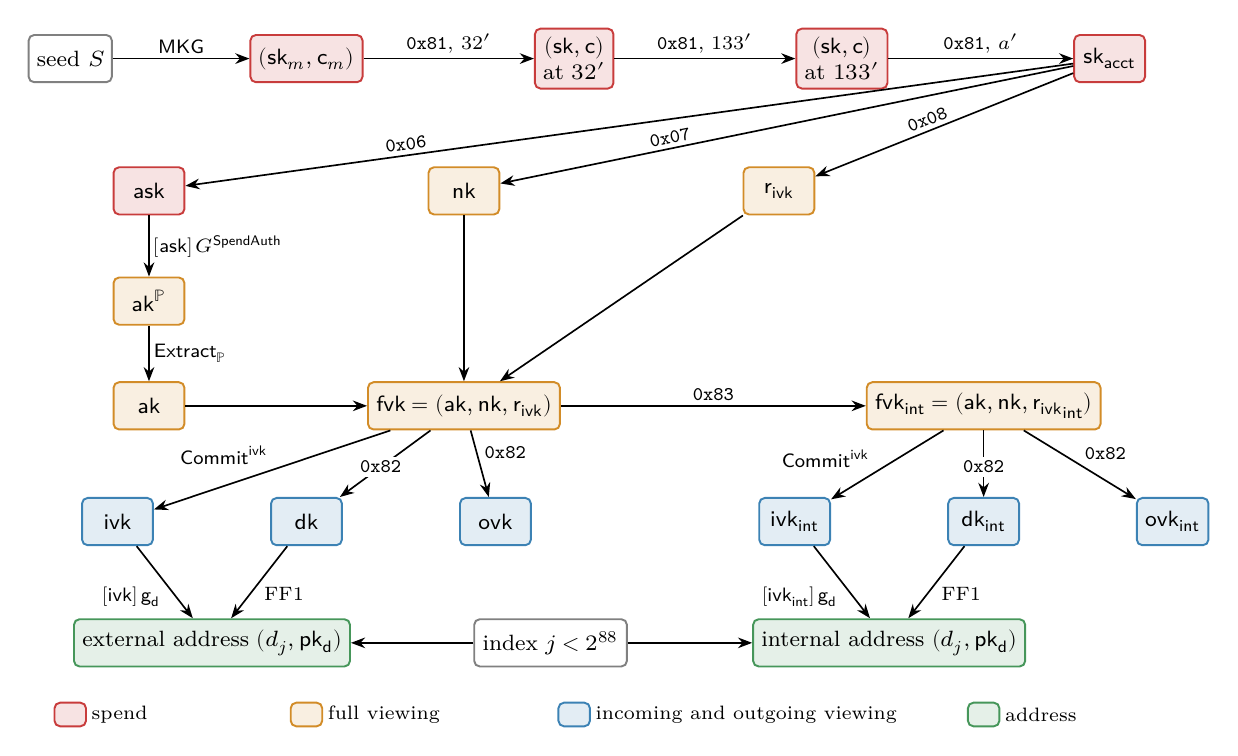
\begin{tikzpicture}[y=0.7cm, font=\footnotesize, >={Stealth[length=1.8mm]}]
% the account path
\node[keyix] (S) at (0,0) {seed $S$};
\node[keykn=tierspend] (m) at (3.0,0) {$(\sksym_m, \mathsf{c}_m)$};
\node[keykn=tierspend] (p1) at (6.4,0) {$(\sksym, \mathsf{c})$\\at $32'$};
\node[keykn=tierspend] (p2) at (9.8,0) {$(\sksym, \mathsf{c})$\\at $133'$};
\node[keykn=tierspend] (acct) at (13.2,0) {$\sksym_{\mathsf{acct}}$};
\draw[keyed] (S) -- node[keylb, above] {$\mathsf{MKG}$} (m);
\draw[keyed] (m) -- node[keylb, above] {$\mathtt{0x81}$, $32'$} (p1);
\draw[keyed] (p1) -- node[keylb, above] {$\mathtt{0x81}$, $133'$} (p2);
\draw[keyed] (p2) -- node[keylb, above] {$\mathtt{0x81}$, $a'$} (acct);
% spend-side secrets
\node[keykn=tierspend] (ask) at (1.0,-2.4) {$\asksym$};
\node[keykn=tierfull] (nk) at (5.0,-2.4) {$\nksym$};
\node[keykn=tierfull] (rivk) at (9.0,-2.4) {$\rivk$};
\draw[keyed] (acct) -- node[keylb, sloped, above, pos=0.75] {$\mathtt{0x06}$} (ask);
\draw[keyed] (acct) -- node[keylb, sloped, above, pos=0.7] {$\mathtt{0x07}$} (nk);
\draw[keyed] (acct) -- node[keylb, sloped, above, pos=0.55] {$\mathtt{0x08}$} (rivk);
% spend validating key
\node[keykn=tierfull] (akP) at (1.0,-4.4) {$\akP$};
\node[keykn=tierfull] (ak) at (1.0,-6.3) {$\aksym$};
\draw[keyed] (ask) -- node[keylb, right] {$[\asksym]\,\GS$} (akP);
\draw[keyed] (akP) -- node[keylb, right] {$\Ext$} (ak);
% full viewing keys
\node[keykn=tierfull] (fvk) at (5.0,-6.3) {$\fvk = (\aksym, \nksym, \rivk)$};
\node[keykn=tierfull] (fvki) at (11.6,-6.3)
  {$\fvk_{\mathsf{int}} = (\aksym, \nksym, \rivk_{\mathsf{int}})$};
\draw[keyed] (ak) -- (fvk);
\draw[keyed] (nk) -- (fvk);
\draw[keyed] (rivk) -- (fvk);
\draw[keyed] (fvk) -- node[keylb, above] {$\mathtt{0x83}$} (fvki);
% per-scope viewing keys
\node[keykn=tierin] (ivk) at (0.6,-8.4) {$\ivk$};
\node[keykn=tierin] (dk) at (3.0,-8.4) {$\dk$};
\node[keykn=tierin] (ovk) at (5.4,-8.4) {$\ovk$};
\node[keykn=tierin] (ivki) at (9.2,-8.4) {$\ivk_{\mathsf{int}}$};
\node[keykn=tierin] (dki) at (11.6,-8.4) {$\dk_{\mathsf{int}}$};
\node[keykn=tierin] (ovki) at (14.0,-8.4) {$\ovk_{\mathsf{int}}$};
\draw[keyed] (fvk) -- node[keylb, above left, pos=0.5] {$\CommitIvk$} (ivk);
\draw[keyed] (fvk) -- node[keylb, fill=white, pos=0.55] {$\mathtt{0x82}$} (dk);
\draw[keyed] (fvk) -- node[keylb, above right, pos=0.5] {$\mathtt{0x82}$} (ovk);
\draw[keyed] (fvki) -- node[keylb, above left, pos=0.62] {$\CommitIvk$} (ivki);
\draw[keyed] (fvki) -- node[keylb, fill=white, pos=0.55] {$\mathtt{0x82}$} (dki);
\draw[keyed] (fvki) -- node[keylb, above right, pos=0.5] {$\mathtt{0x82}$} (ovki);
% addresses
\node[keykn=tierrecv] (addr) at (1.8,-10.6) {external address $(d_j, \pkd)$};
\node[keykn=tierrecv] (addri) at (10.4,-10.6) {internal address $(d_j, \pkd)$};
\node[keyix] (j) at (6.1,-10.6) {index $j < 2^{88}$};
\draw[keyed] (dk) -- node[keylb, below right] {FF1} (addr);
\draw[keyed] (ivk) -- node[keylb, below left] {$[\ivk]\,\gd$} (addr);
\draw[keyed] (j) -- (addr);
\draw[keyed] (dki) -- node[keylb, below right] {FF1} (addri);
\draw[keyed] (ivki) -- node[keylb, below left] {$[\ivk_{\mathsf{int}}]\,\gd$} (addri);
\draw[keyed] (j) -- (addri);
% legend
\foreach \c/\t/\x in {tierspend/spend/0.0, tierfull/full viewing/3.0,
    tierin/incoming and outgoing viewing/6.4, tierrecv/address/11.6} {
  \node[keykn=\c, minimum width=4mm, minimum height=3mm, inner sep=0pt]
    (lg) at (\x,-11.9) {};
  \node[keylb, anchor=west] at (lg.east) {\t};
}
\end{tikzpicture}}
\end{frame}

% ====================================================================
\divider{Someone pays you}

\begin{frame}{The note}
The sender creates
\[
n = \bigl((d, \pkd),\ v,\ \rho,\ \psi,\ \rcm\bigr)
\]
with $v$ the amount in zatoshi and $\rho := \nfsym^{\mathrm{old}}$, the
nullifier
the same Action spends. From one fresh seed $\rseed$:
\begin{align*}
\esk &:= \mathrm{ToScalar}\bigl(\PRFx{\rseed}([\mathtt{04}] \,\|\, \rho)\bigr) \\
\psi &:= \mathrm{ToBase}\bigl(\PRFx{\rseed}([\mathtt{09}] \,\|\, \rho)\bigr) \\
\rcm &:= \mathrm{ToScalar}\bigl(\PRFx{\rseed}([\mathtt{0B}] \,\|\, \gd \,\|\, \pkd \,\|\, v \,\|\, \rho \,\|\, \psi)\bigr)
\end{align*}
\types{One seed fixes the note's randomness and the encryption key; the
recipient can re-derive all three.}
\end{frame}

\begin{frame}{The note commitment}
\begin{align*}
\cmsym &:= \NoteCommit_{\rcm}(\gd, \pkd, v, \rho, \psi) \\
  &\phantom{:}= \SinPt(\gd \,\|\, \pkd \,\|\, v \,\|\, \rho \,\|\, \psi) + [\rcm]\,H_{\mathrm{cm}} \\
\cmx &:= \Ext(\cmsym)
\end{align*}
\vfill
\begin{itemize}\itemsep6pt
\item \textbf{Hiding}: for uniform $\rcm$, $\cmsym$ is a uniform point, whatever
  the note.
\item \textbf{Binding}: two notes with one $\cmx$ give a discrete-log relation
  among the generators.
\item $\cmx$ is appended to the note commitment tree; the note itself never
  appears.
\end{itemize}
\end{frame}

\begin{frame}{Encryption to the address}
\[
\epk := [\esk]\,\gd, \qquad s := [\esk]\,\pkd,
\]
\[
K := \mathrm{BLAKE2b\text{-}256}(\texttt{Zcash\_OrchardKDF},\, s \,\|\, \epk)
\]
\[
C_{\mathrm{enc}} := \mathrm{ChaCha20\text{-}Poly1305}_K\bigl(
  \mathtt{0x03} \,\|\, d \,\|\, v \,\|\, \rseed \,\|\, \mathsf{memo}\bigr)
  \quad \text{\grey{($580$ bytes)}}
\]
\vfill
The recipient holds $\ivk$ with $\pkd = [\ivk]\,\gd$, so
\[
[\ivk]\,\epk = [\ivk \cdot \esk]\,\gd = [\esk]\,\pkd = s .
\]
Diffie--Hellman on a per-address base: without $\esk$, only $\ivk$ recovers
$K$.
\end{frame}

\begin{frame}{What reaches the chain}
\begin{center}
\scalebox{1.1}{\ActionBox[cmx]}
\end{center}
\small
Per Action: $\cvnet$, $\nfsym$, $\rk$, $\cmx$, $\epk$, $C_{\mathrm{enc}}$,
$C_{\mathrm{out}}$ ($820$ bytes). Nothing names the recipient.
\end{frame}

% ====================================================================
\divider{Scanning}

\begin{frame}{Compact blocks}
A light wallet does not download full transactions. Per Action it receives
\[
\bigl(\nfsym,\ \cmx,\ \epk,\ C_{\mathrm{enc}}[0{:}52]\bigr)
  \quad \text{\grey{$32 + 32 + 32 + 52 = 148$ bytes}}
\]
\vfill
The first $52$ bytes of the plaintext are
$\mathtt{leadByte} \,\|\, d \,\|\, v \,\|\, \rseed$: everything but the memo.
\vfill
The memo, the tag and $C_{\mathrm{out}}$ are fetched only for the wallet's
own transactions.
\end{frame}

\begin{frame}{Trial decryption}
For every Action, with the wallet's $\ivk$:
\begin{enumerate}\itemsep5pt
\item $s := [\ivk]\,\epk$, \quad $K := \mathrm{KDF}(s, \epk)$, \quad decrypt
  $52$ bytes;
\item $\gd := \GroupHash(d)$, \quad $\pkd := [\ivk]\,\gd$;
\item re-derive $\esk$, $\psi$, $\rcm$ from $\rseed$ and $\rho = \nfsym$ of the
  same Action;
\item accept only if $[\esk]\,\gd = \epk$ \ and \
  $\Ext(\NoteCommit_{\rcm}(\dots)) = \cmx$.
\end{enumerate}
\vfill
An Action for someone else decrypts to garbage and fails step 4. An
accepted note is the unique opening of $\cmx$: the sender cannot make the
wallet accept a note it cannot later spend.
\end{frame}

\begin{frame}{Keeping a witness}
\begin{columns}[c]
\begin{column}{0.44\textwidth}
\centering
\TreeFig[path]
\end{column}
\begin{column}{0.54\textwidth}
\small
The note's $\cmx$ sits at position $\mathsf{pos}$ of a depth-$32$ tree.
With $h_t := \MCRH(31 - t, \cdot, \cdot)$:
\[
a_0 := \cmx,\quad a_{t+1} := \begin{cases} h_t(a_t, s_t) & b_t = 0 \\ h_t(s_t, a_t) & b_t = 1 \end{cases}
\]
Valid path: $a_{32} = \mathit{rt}$, the anchor.
\end{column}
\end{columns}
\vfill
Every sibling $s_t$ is a function of the $\cmx$ values appended so far: the
wallet updates the path from the blocks it scans and never reveals
$\mathsf{pos}$.
\end{frame}

\begin{frame}{Watching for spends}
The wallet computes its note's nullifier once:
\[
\nfsym := \Ext\bigl([(\mathsf{PoseidonHash}(\nksym, \rho) + \psi) \bmod \pP]\,\KO + \cmsym\bigr)
\]
and marks the note spent when $\nfsym$ appears in a scanned block.
\vfill
\begin{itemize}\itemsep5pt
\item Deterministic: one note, one nullifier.
\item Unlinkable: without $\nksym$ it looks random.
\item The wallet now holds everything a spend needs: the note, $\mathsf{pos}$,
  the path, an anchor.
\end{itemize}
\end{frame}

% ====================================================================
\divider{Spending}

\begin{frame}{The spend side of an Action}
\begin{align*}
\nfsym^{\mathrm{old}} &:= \DNf_{\nksym}(\rho, \psi, \cmsym) && \text{published} \\
\rsk := \asksym + \alpha, \quad \rk &:= \akP + [\alpha]\,\GS && \text{fresh } \alpha \text{ per Action} \\
\cvnet &:= [v^{\mathrm{old}} - v^{\mathrm{new}}]\,\VO + [\rcv]\,\RO && \text{fresh } \rcv
\end{align*}
\vfill
\begin{itemize}\itemsep5pt
\item $\rk$ is a uniform point: two spends by one key are unlinkable.
\item $\cvnet$ is a uniform point: the amount is hidden, and commitments add up.
\end{itemize}
\end{frame}

\begin{frame}{The output side}
The new note goes to the payee, change to an internal address of the payer;
each
with
\[
\rho^{\mathrm{new}} := \nfsym^{\mathrm{old}}
\]
so every created note carries a unique $\rho$. Unused sides are dummy notes
of value $0$: every Action has exactly one spend and one output.
\vfill
\begin{center}\small
\begin{tabular}{@{}lrrr@{}}
\toprule
Action & $v^{\mathrm{old}}$ & $v^{\mathrm{new}}$ & $v^{\mathrm{old}} - v^{\mathrm{new}}$ \\
\midrule
note $\to$ payee & $7$ ZEC & $5$ ZEC & $2$ ZEC \\
dummy $\to$ change & $0$ & $1.9999$ ZEC & $-1.9999$ ZEC \\
\midrule
$\vbal$ (the fee) & & & $0.0001$ ZEC \\
\bottomrule
\end{tabular}
\end{center}
\end{frame}

\begin{frame}{What the proof asserts}
For public $(\mathit{rt}, \cvnet, \nfsym^{\mathrm{old}}, \rk, \cmx,
\text{flags})$,
the prover knows a witness such that:
\begin{enumerate}\itemsep3pt
\item the old note opens $\cmsym^{\mathrm{old}}$, and $\cmsym^{\mathrm{old}}$
  has a valid path to $\mathit{rt}$ (if $v^{\mathrm{old}} \ne 0$);
\item $\nfsym^{\mathrm{old}} = \DNf_{\nksym}(\rho, \psi,
  \cmsym^{\mathrm{old}})$;
\item $\rk = \akP + [\alpha]\,\GS$, and $\pkd^{\mathrm{old}} =
  [\CommitIvk_{\rivk}(\aksym, \nksym)]\,\gd^{\mathrm{old}}$;
\item $\cvnet = [v^{\mathrm{old}} - v^{\mathrm{new}}]\,\VO + [\rcv]\,\RO$;
\item the new note opens $\cmx$, with $\rho^{\mathrm{new}} =
  \nfsym^{\mathrm{old}}$;
\item the flags hold (spends, outputs, cross-address).
\end{enumerate}
\vfill
One Halo~2 proof for all Actions of the bundle.
\end{frame}

\begin{frame}{Signatures}
Every signature signs $\mathsf{SigHash}$, a BLAKE2b digest of the transaction
without its proofs and signatures.
\vfill
\begin{itemize}\itemsep8pt
\item \textbf{Spend authorisation}, per Action: RedPallas under $\rsk$, checked
  against $\rk$. Only a holder of $\asksym$ can produce it.
\item \textbf{Binding}, per bundle:
\[
\mathsf{bsk} := \sum_i \rcv_i, \qquad
\mathsf{bvk} := \sum_i \cvsym_i - [\vbal]\,\VO
\]
  RedPallas under $\mathsf{bsk}$, checked against $\mathsf{bvk}$.
\end{itemize}
\end{frame}

% ====================================================================
\divider{Verification}

\begin{frame}{What a node checks}
\begin{center}
\renewcommand{\arraystretch}{1.35}
\begin{tabular}{@{}ll@{}}
\toprule
check & guarantees \\
\midrule
the proof, on the public fields & statement 1--6 for every Action \\
$\mathit{rt}$ is a past anchor & the spent note exists \\
$\nfsym \notin$ nullifier set & not spent before \\
spend signature under $\rk$ & the owner authorised it \\
binding signature under $\mathsf{bvk}$ & value is conserved \\
\bottomrule
\end{tabular}
\end{center}
\vfill
Then: every $\nfsym$ joins the set, every $\cmx$ joins the tree. No step
reads a note.
\end{frame}

\begin{frame}{Why the binding signature enforces balance}
Commitments add:
\[
\sum_i \cvsym_i = \Bigl[\sum_i (v^{\mathrm{old}}_i - v^{\mathrm{new}}_i)\Bigr]\VO
  + \Bigl[\sum_i \rcv_i\Bigr]\RO
\]
so
\[
\mathsf{bvk} - [\mathsf{bsk}]\,\RO = \Bigl[\sum_i (v^{\mathrm{old}}_i - v^{\mathrm{new}}_i) - \vbal\Bigr]\,\VO .
\]
\vfill
A valid signature proves knowledge of $b$ with $\mathsf{bvk} = [b]\,\RO$.
If the values did not balance, $b$ would yield $\log_{\RO} \VO$, a relation
between two hashed generators: infeasible.
\vfill
\types{The sum is below $2^{80} \ll \pV$, so balance modulo $\pV$ is balance
over the integers.}
\end{frame}

% ====================================================================
\divider{How Halo 2 proves}
\begin{frame}{The claim becomes a table}
``I know $x$ with $x^3 + x + 5 = 35$'' over $\F_{97}$; the witness $x = 3$:
\[
3 \xrightarrow{\ \text{square}\ } 9 \xrightarrow{\ \times 3\ } 27
  \xrightarrow{\ + 3\ } 30 \xrightarrow{\ + 5\ } 35 .
\]
One operation per row, one gate equation on every row:
\[
q_M\, a\, b + q_L\, a + q_R\, b + q_O\, c + q_C + \mathrm{PI} = 0
\]
\types{every cell in $\F_{97}$.}
\begin{center}\small
\begin{tabular}{@{}c ccc ccccc c l@{}}
\toprule
& \multicolumn{3}{c}{advice} & \multicolumn{5}{c}{fixed} & instance & \\
\cmidrule(lr){2-4}\cmidrule(lr){5-9}\cmidrule(lr){10-10}
row & $a$ & $b$ & $c$ & $q_M$ & $q_L$ & $q_R$ & $q_O$ & $q_C$
  & $\mathrm{PI}$ & \\
\midrule
0 & 3 & 3 & 9 & 1 & 0 & 0 & $-1$ & 0 & 0 & $x \cdot x = x^2$ \\
1 & 9 & 3 & 27 & 1 & 0 & 0 & $-1$ & 0 & 0 & $x^2 \cdot x = x^3$ \\
2 & 27 & 3 & 30 & 0 & 1 & 1 & $-1$ & 0 & 0 & $x^3 + x = s$ \\
3 & 30 & 0 & 0 & 0 & 1 & 0 & 0 & 5 & $-35$ & $s + 5 = 35$ \\
\bottomrule
\end{tabular}
\end{center}
Advice: the prover's secret trace. Fixed: the circuit. Instance: the public
$35$.
Copy constraints wire the rows; range checks are lookups into a table.
\end{frame}

\begin{frame}{Equal values must be wired together}
\begin{center}
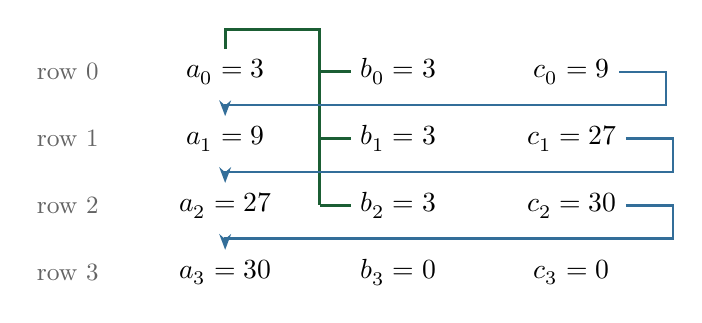
\begin{tikzpicture}[x=1cm,y=1cm]
\foreach \i/\av/\bv/\cvv in {0/3/3/9,1/9/3/27,2/27/3/30,3/30/0/0}{
  \node[labeltext] at (0,-.85*\i) {row $\i$};
  \node (a\i) at (2,-.85*\i) {$a_{\i}=\av$};
  \node (b\i) at (4.2,-.85*\i) {$b_{\i}=\bv$};
  \node (c\i) at (6.4,-.85*\i) {$c_{\i}=\cvv$};
}
\draw[very thick,arb] (a0.north) -- ++(0,.25) -| (3.2,0) -- (3.2,-1.7);
\foreach \i in {0,1,2} \draw[very thick,arb] (3.2,-.85*\i)--(b\i.west);
\draw[flow,tierin!85!black] (c0.east) -- ++(.6,0) -- ++(0,-.42) -| (a1.north);
\draw[flow,tierin!85!black] (c1.east) -- ++(.6,0) -- ++(0,-.42) -| (a2.north);
\draw[flow,tierin!85!black] (c2.east) -- ++(.6,0) -- ++(0,-.42) -| (a3.north);
\end{tikzpicture}
\end{center}
\vfill
Equal numbers in a table are not a constraint. These \emph{copy
constraints} are enforced separately, by a permutation argument.
\end{frame}

\begin{frame}{Give the rows multiplicative labels}
\begin{columns}[c]
\begin{column}{0.42\textwidth}
\centering
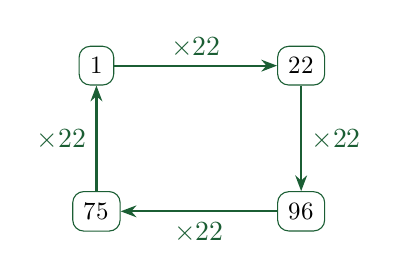
\begin{tikzpicture}[x=1cm,y=1cm]
\node[box] (a) at (0,1.25) {$1$};
\node[box] (b) at (2.6,1.25) {$22$};
\node[box] (c) at (2.6,-.6) {$96$};
\node[box] (d) at (0,-.6) {$75$};
\draw[flow] (a)--node[above] {$\times 22$} (b);
\draw[flow] (b)--node[right] {$\times 22$} (c);
\draw[flow] (c)--node[below] {$\times 22$} (d);
\draw[flow] (d)--node[left] {$\times 22$} (a);
\end{tikzpicture}
\end{column}
\begin{column}{0.54\textwidth}
\[
\omega = 22,\qquad \omega^2 = 96 = -1,\qquad \omega^4 = 1
\]
\[
H = \{1, 22, 96, 75\} \subset \F_{97}
\]
Row $i$ gets the label $\omega^i$: a cycle of field values.
\end{column}
\end{columns}
\end{frame}

\begin{frame}{Rows become polynomials}
Row $i$ lives at $\omega^i \in H$. Interpolate each column:
\[
a(1) = 3,\ a(22) = 9,\ a(96) = 27,\ a(75) = 30
\ \Longrightarrow\
a(X) = 90 + 61X + 22X^2 + 24X^3
\]
\[
G(X) := q_M a b + q_L a + q_R b + q_O c + q_C + \mathrm{PI}
\]
\types{$a, b, c, q_\bullet, \mathrm{PI} \in \F_{97}[X]$ of degree $< 4$; $G \in
\F_{97}[X]$ of degree $\le 9$.}
\vfill
\[
\GZH(X) := \prod_{h \in H}(X - h) = X^4 - 1
\]
\[
\text{every gate holds}
\iff G \text{ vanishes on } H
\iff \GZH \mid G
\iff G = t \cdot \GZH
\]
\vfill
A correct computation \emph{is} a polynomial identity. A wrong one cannot be:
the lie $x^2 = 10$ in row $0$ leaves a remainder $24\,(1 + X + X^2 + X^3) \ne
0$.
\end{frame}

\begin{frame}{One random point}
\begin{center}
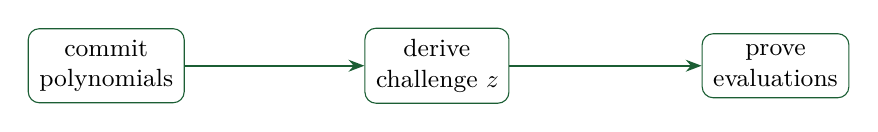
\begin{tikzpicture}[x=1cm,y=1cm]
\node[box] (c) at (0,0) {commit\\polynomials};
\node[box] (z) at (4.2,0) {derive\\challenge $z$};
\node[box] (o) at (8.5,0) {prove\\evaluations};
\draw[flow] (c)--(z); \draw[flow] (z)--(o);
\end{tikzpicture}
\end{center}
\begin{enumerate}\itemsep3pt
  \item The prover \emph{commits} to $a, b, c$ and $t$.
  \item The challenge $z := \mathsf{H}(\text{transcript})$ --- Fiat--Shamir.
  \item The prover opens $a(z), b(z), c(z), t(z)$.
  \item The verifier checks one equation:
  \[
  G(z) \overset{?}{=} t(z)\, \GZH(z)
  \]
\end{enumerate}
\types{$z \in \F_{97}$ in the toy; $z \in \Fpp$ in the protocol.}
\vfill
Honest, $z = 20$: $G(20) = 75 = 67 \cdot 46$. \quad
The row-$0$ lie: $G^{*}(20) = 20 \ne 64$.
\vfill
A false identity is frozen before $z$ is drawn; it survives only if $z$
is one of its few roots.
\end{frame}

\begin{frame}{A nonzero polynomial has few roots}
The remainder $D(X) = 24\,(1 + X + X^2 + X^3)$ over $\F_{97}$: zeros at
$22, 75, 96$ only.
\begin{center}
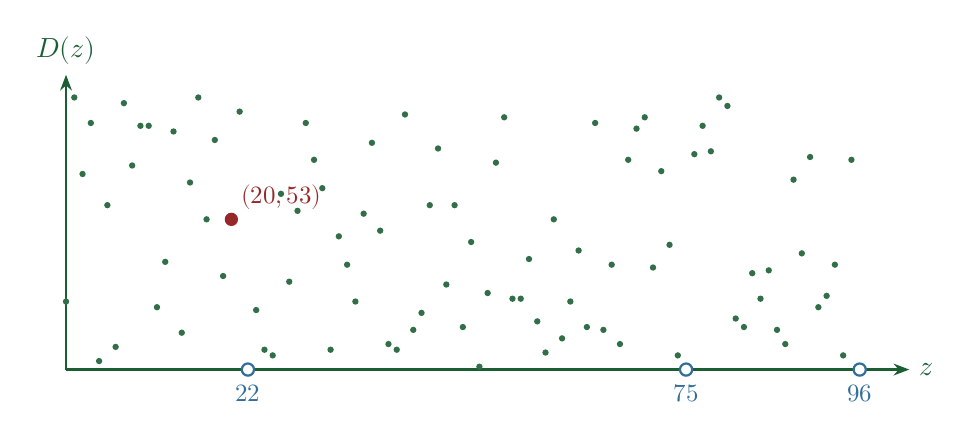
\begin{tikzpicture}[x=.105cm,y=.036cm]
\draw[flow] (0,0)--(102,0) node[right] {$z$};
\draw[flow] (0,0)--(0,104) node[above] {$D(z)$};
\foreach \x in {0,...,96}{
  \pgfmathtruncatemacro{\square}{mod(\x*\x,97)}
  \pgfmathtruncatemacro{\cube}{mod(\square*\x,97)}
  \pgfmathtruncatemacro{\residue}{mod(24*(1+\x+\square+\cube),97)}
  \fill[arb!90] (\x,\residue) circle[radius=1.15pt];
}
\foreach \x in {22,75,96}{
  \draw[tierin!85!black,thick,fill=white] (\x,0) circle[radius=2.2pt];
  \node[below,font=\small,text=tierin!85!black] at (\x,-2) {$\x$};
}
\fill[arbred] (20,53) circle[radius=2.4pt];
\node[above right,font=\small,text=arbred] at (20,53) {$(20, 53)$};
\end{tikzpicture}
\end{center}
For uniform $z$ this cheat passes with probability $3/97$; over the
protocol's field, about $2^{-240}$.
\end{frame}

\begin{frame}{Committing to a polynomial}
\[
P := \ip{\vec a}{\vec G} + [r]\,H,\qquad
\vec a = (a_0, \dots, a_{d-1}),\quad \vec G \text{ independent points}
\]
\[
a(z) = \ip{\vec a}{\vec b},\qquad \vec b := (1, z, z^2, \dots, z^{d-1})
\]
\types{$a_i, r, z \in \Fpp$; $\vec G, H, P \in \Vs$, the Vesta curve, whose
scalar field is $\Fpp$.}
\vfill
\begin{itemize}\itemsep6pt
  \item A Pedersen commitment to the coefficient vector: hiding, binding.
  \item Opening at $z$ is an inner product with a public vector.
  \item The problem: convince the verifier of $\ip{\vec a}{\vec b} = v$
    in fewer than $d$ group elements, without sending $\vec a$.
\end{itemize}
\end{frame}

\begin{frame}{The inner-product argument: one fold}
Split every vector in half and publish two cross terms:
\begin{align*}
L &:= \ip{\Glo{\vec a}}{\Ghi{\vec G}} + [\ell]\,H + [\ip{\Glo{\vec a}}{\Ghi{\vec b}}]\,U, \\
R &:= \ip{\Ghi{\vec a}}{\Glo{\vec G}} + [r_R]\,H + [\ip{\Ghi{\vec a}}{\Glo{\vec b}}]\,U .
\end{align*}
Challenge $u$; both sides fold:
\[
\vec a' := u\,\Glo{\vec a} + u^{-1}\Ghi{\vec a}, \qquad
\vec G' := u^{-1}\Glo{\vec G} + u\,\Ghi{\vec G}, \qquad
\vec b' := u^{-1}\Glo{\vec b} + u\,\Ghi{\vec b}
\]
\[
P + [v]\,U + [u^2]\,L + [u^{-2}]\,R
= \ip{\vec a'}{\vec G'} + [r + u^2 \ell + u^{-2} r_R]\,H + [\ip{\vec a'}{\vec b'}]\,U
\]
\types{$u \in \Fpp^{\times}$; $L, R, U, H \in \Vs$; $\ell, r_R \in \Fpp$.}
\vfill
The same claim at half the length. The verifier folds $\vec G$ and $\vec b$
itself and never sees $\vec a$.
\end{frame}

\begin{frame}{The recursion}
After $k = \log_2 d$ rounds every vector has length $1$. The proof: $2k$
points $(L_j, R_j)$, one scalar $a$, one blinder $r^{*}$.
\[
P + [v]\,U + \sum_{j=1}^{k}\bigl([u_j^2]\,L_j + [u_j^{-2}]\,R_j\bigr)
\overset{?}{=} [a]\,G^{(0)} + [r^{*}]\,H + [a\cdot b^{(0)}]\,U
\]
\types{$a, b^{(0)}, r^{*}, u_j \in \Fpp$; $G^{(0)}, L_j, R_j \in \Vs$.}
\vfill
\begin{itemize}\itemsep6pt
  \item The scalar $b^{(0)} = \prod_j (u_j^{-1} + u_j\, z^{2^{j-1}})$, with
    $u_1$
    the last challenge: logarithmic work.
  \item The point $G^{(0)} = \ip{\vec s}{\vec G}$: one multi-scalar
    multiplication,
    shared across a batch of proofs.
  \item Binding: two openings would give a discrete-log relation among
    $\vec G, H$; an extractor rewinds three challenges per round.
\end{itemize}
\end{frame}

\begin{frame}{The Orchard circuit}
\begin{itemize}\itemsep6pt
  \item Size: $2^{11}$ rows, $10$ advice columns; arithmetic over $\Fpp$ so
    Pallas points $\cmsym, \rksym, \cvsym$ are native; commitments on Vesta.
  \item Gadgets: Sinsemilla (commitments, tree), Poseidon (nullifier),
    elliptic-curve arithmetic, lookups for range checks.
  \item The instance: anchor, $\cvsym$, $\nfsym$, $\rksym$, $\cmx$, flags.
  \item Generators from a hash: no trusted setup, no ceremony.
  \item Proof size $2720 + 2272\,a$ bytes for $a$ Actions: $4992$ for one.
\end{itemize}
\vfill
Every clause of the statement is a set of rows; one proof, one random
point, one inner-product argument.
\end{frame}

% ====================================================================
\begin{frame}{The whole path}
\begin{center}
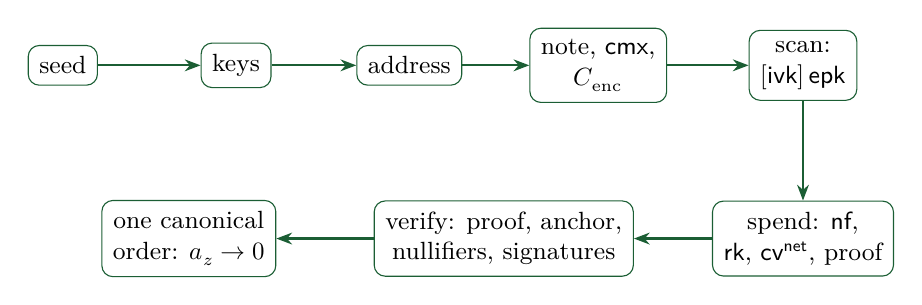
\begin{tikzpicture}[x=1cm,y=1cm, every node/.style={font=\small}]
\node[box] (s) at (0,0) {seed};
\node[box] (k) at (2.2,0) {keys};
\node[box] (a) at (4.4,0) {address};
\node[box] (n) at (6.8,0) {note, $\cmx$,\\$C_{\mathrm{enc}}$};
\node[box] (c) at (9.4,0) {scan:\\$[\ivk]\,\epk$};
\node[box] (sp) at (9.4,-2.2) {spend: $\nfsym$,\\$\rk$, $\cvnet$, proof};
\node[box] (v) at (5.6,-2.2) {verify: proof, anchor,\\nullifiers, signatures};
\node[box] (o) at (1.6,-2.2) {one canonical\\order: $a_z \to 0$};
\draw[flow] (s)--(k); \draw[flow] (k)--(a); \draw[flow] (a)--(n);
\draw[flow] (n)--(c); \draw[flow] (c)--(sp); \draw[flow] (sp)--(v);
\draw[flow] (v)--(o);
\end{tikzpicture}
\end{center}
\vfill
The verifier learns that every check passes, the fee, the anchor and the
flags, and nothing about the notes.
\end{frame}

\end{document}
